\section{Stability}

\begin{frame}{Stability in Discrete Time}

A discrete system is stable iff all eigenvalues have magnitude less than 1. If any eigenvalue has magnitude greater than 1, then any state vector with a nonzero corresponding eigenvector component will have that component repeatedly magnified.

    For example: \(x[t+1] = 2 x[t]\)

\end{frame}

\begin{frame}{Stability in Discrete Time}
A discrete system is stable iff
    \[
        \forall x \in eig(A) : |x| < 1
    \]

The eigenvectors form a basis (called the eigenbasis) which spans the entire space if A is full rank. (can you prove this?)

If any eigenvalue has magnitude greater than 1, then any state vector with a nonzero corresponding eigenvector component will have that component repeatedly magnified.
\end{frame}

\begin{frame}{Stability in Discrete Time}

How do the eigenvalues govern system dynamics?

    If initial state is x(0), and there's no control input, the \(n\)th state is
    \[
        x(n) = A^n x(0)
    \]

    If any eigenvalue of \(A\) is larger in magnitude than \(1\), it ``blows up'' through repeated exponentiation - the system destabilizes!
\end{frame}

\begin{frame}{Stability in Discrete Time}
    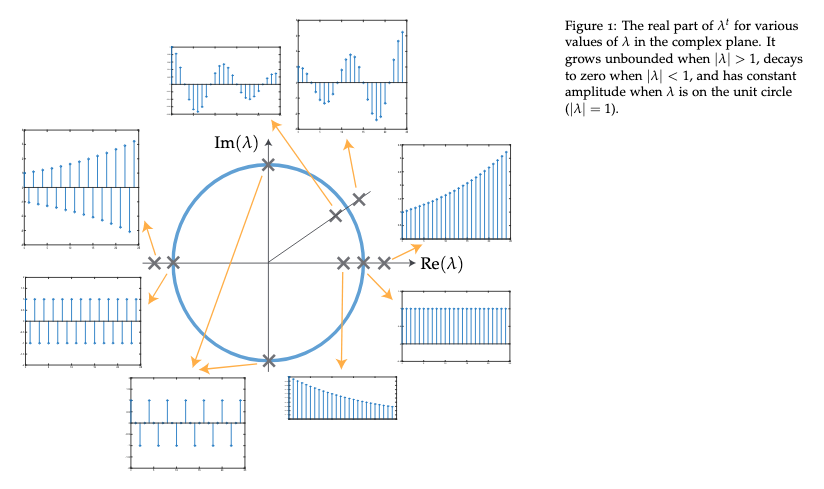
\includegraphics[width=\textwidth]{./images/eigenvalues-on-the-unit-circle}
\end{frame}

\begin{frame}{Stability in Continuous Time}

A continuous system is stable iff the real parts of all eigenvalues are negative. If any eigenvalue is positive, then any state vector with a nonzero corresponding eigenvector component will have that component grow exponentially to infinity.

    For example: \(\ddt{}x(t) = 2\,x(t)\)

\end{frame}

\begin{frame}{Stability in Continuous Time}

    \[
        \ddt{} x(t) = a x(t) + b u(t)
    \]

    \[
        x(t) = e^{at} x(0) + b \int_0^t e^{a(t - s)} u(s) \,\differential s
    \]

    For scalar case, system is stable if \(\mathrm{Re}\{a\} < 0\) and not stable if \(\mathrm{Re}\{a\} > 0\).

    By careful application of diagonalization, we get the same result for the eigenvalues of \(A\) in the matrix case. 

\end{frame}

\begin{frame}{Stability in Continuous Time}
    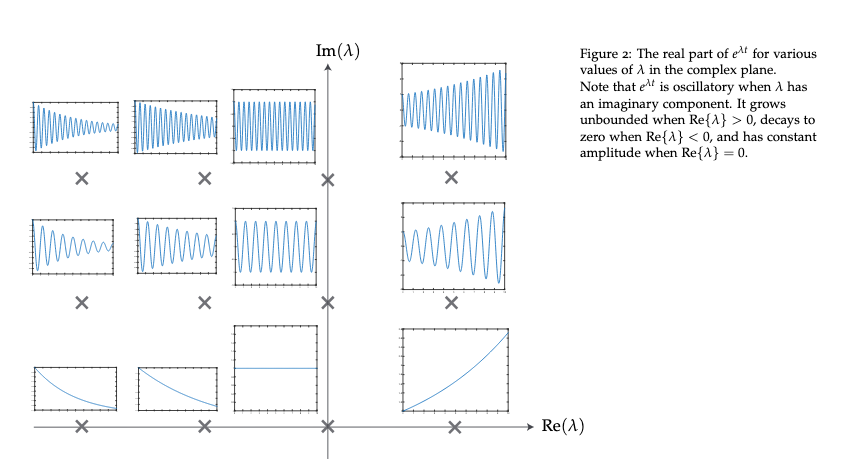
\includegraphics[width=\textwidth]{./images/cont-stability}
\end{frame}

\begin{frame}{Stability in Continuous Time}
How do the eigenvalues govern system dynamics?

    If initial state is \(\vec x(0)\), and there's no control input, state at time \(t\) is
    \[
        \vec x(t) = e^{At} \vec x(0)
    \]
    If any eigenvalue of \(A\) is larger in magnitude than \(1\), it ``blows up'' through repeated exponentiation --- the system destabilizes!
\end{frame}


\begin{frame}{Stability Through State Feedback}

\begin{columns}[T] % align columns
\begin{column}{.48\textwidth}
%\color{red}\rule{\linewidth}{4pt}
%
%Left Part
    \begin{itemize}
        \item If we add a feedback path (modifying the input values with the state) our state update equation changes \[ \vec x(t + 1) = (A + BK) \vec x(t)\]
        \item What determines the stability of this new system?
    \end{itemize}

\end{column}%
\hfill%
\begin{column}{.48\textwidth}
    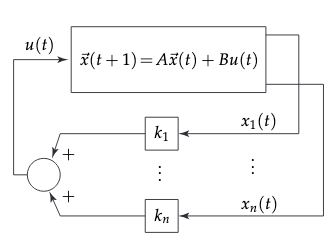
\includegraphics[width=\textwidth]{./images/block-diagram-of-system.png}

\end{column}%
\end{columns}

\end{frame}

\begin{frame}{State Feedback}
    \begin{itemize}
        \item 
By designing K, we can give our system specific dynamic properties
            \begin{itemize}
        \item 
Can analyze and design the way its state changes over time
            \end{itemize}
        \item 
If our “open-loop” system is unstable, choosing the right values of K can make it stable!
        \item 
Is this always possible?
    \end{itemize}
\end{frame}

\begin{frame}{Example: Controllability and Stability}
    \[
        \vec x[t + 1] = \begin{bmatrix}
            -5 & 0 \\
            7 & 6
            \end{bmatrix} \vec x[t] +  \begin{bmatrix} 2 \\ -1\end{bmatrix} u[t]
    \]
    \[
        \vec y[t] = \begin{bmatrix} 1 & 1 \end{bmatrix} \vec x[t]
   \]

   Controllable? 
            \onslide<2->{{\bfseries Yes}}
   
    Stable for \(u[t] = 0\)?
            \onslide<3->{{\bfseries No}}
\end{frame}

\begin{frame}{Upper Triangularization}

    \begin{itemize}
        \item
Recall that not all square matrices are diagonalizable
            \begin{itemize}
        \item
           An \(n \times n\) matrix is diagonalizable iff has \(n\) linearly independent eigenvectors
            \end{itemize}
        \item
However, all square matrices can be brought into upper triangular form
        \item
I’ll walk through the proof from the notes
        \item
(But I’m not sure how useful this will be / how they would ask questions about this on the test)
        \item
(So if people want to I can instead start taking questions on SVD, time- and frequency-domain analysis of RLC circuits, and phasors)
    \end{itemize}
\end{frame}

\begin{frame}{Upper Triangularization Proof}
    \begin{itemize}
        \item What are we trying to prove?
            \begin{itemize}
                \item
                    Remember that if \(M\) is diagonalizable, this means that there exists a matrix \(P\) such that \(PMP^{-1}\) was diagonal
                \item In our case, we want to prove that for any square matrix \(A\), there exists a matrix \(T\) such that \(TAT^{-1}\) is upper triangular
            \end{itemize}
        \item We will proceed by induction
        \item First prove a base case (a \(1 \times 1\) matrix must be upper triangular)
        \item  Prove that if there exists such a matrix \(T_0\) for a \(k \times k\) matrix, then there exists the matrix \(T\) for a size \((k+1) \times (k+1)\) matrix
    \end{itemize}
\end{frame}

\begin{frame}{Upper Triangularization Proof}

\begin{columns}[T] % align columns
\begin{column}{.38\textwidth}
%\color{red}\rule{\linewidth}{4pt}
%
%Left Part
    \begin{itemize}
        \item Clearly a \(1 \times 1\) matrix is upper triangular
        \item 
            First we choose one arbitrary eigenvalue / eigenvector pair, choose an orthonormal basis for \(\mathbb R^n\) (with Gram-Schmidt), then define \(V\) formed with those vectors.
    \end{itemize}

\end{column}%
\hfill%
\begin{column}{.66\textwidth}
    We can upper triangularize \((k+1) \times (k+1)\) matrices if we assume that \(k \times k\) matrices can be upper triangularized.

    To show this, let \(A\) be an arbitrary \((k+1) \times (k + 1)\) matrix and let \(\lambda, \vec v\) by an eigenvalue/vector pair: \(A \vec v = \lambda \vec v\).
    Normalize \(\vec v\) so that \(\lVert \vec v \rVert = 1\) and choose \(k\) other vectors \(\vec v_1, \ldots, \vec v_k \in \mathbb R^{k+1}\) such that \(\{\vec v, \vec v_1, \ldots, \vec v_k\}\) is an orthonormal basis for \(\mathbb R^{k+1}\). Then the \((k+1) \times (k+1)\) matrix \(V \coloneqq \begin{bmatrix} \vec v & \vec v_1 & \cdots  &\vec v_k \end{bmatrix}\) is orthogonal, \emph{i.e.} 
        \( V^{-1} = V^T
        \).



\end{column}%
\end{columns}


\end{frame}
